\documentclass{article}


% load package with some of the available options - you may not need this!
\usepackage[framed,autolinebreaks,useliterate]{mcode}

% for checklist
\usepackage{enumitem,amssymb}
\newlist{todolist}{itemize}{2}
\setlist[todolist]{label=$\square$}
\usepackage{pifont}
\newcommand{\cmark}{\ding{51}}%
\newcommand{\xmark}{\ding{55}}%
\newcommand{\done}{\rlap{$\square$}{\raisebox{2pt}{\large\hspace{1pt}\cmark}}%
\hspace{-2.5pt}}
\newcommand{\wontfix}{\rlap{$\square$}{\large\hspace{1pt}\xmark}}
\usepackage{subcaption}

% something NOT relevant to the usage of the package.
\usepackage{graphicx}
\usepackage{url,textcomp}
\setlength{\parindent}{0pt}
\setlength{\parskip}{18pt}
\title{ECTA Homework 3\\Shape Matching Problem}
\author{\color{blue}Erick Kramer, Mihir Patil\\ \texttt{\color{blue}erick.romero@smail.inf.h-brs.de , mihir.patil@smail.inf.h-brs.de}}
% //////////////////////////////////////////////////

\begin{document}

\maketitle
\begin{center}
	\begin{minipage}{1\linewidth}
		\centering
			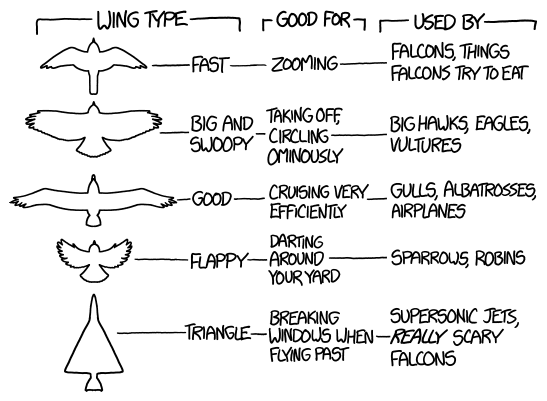
\includegraphics[scale=0.6]{img/wingtypes.png}
	\end{minipage}
\end{center}

To optimize wings, it is useful to start with known designs and then adjust them to specific tasks. How to convert from one representation to another? In this assignment you will convert the 4-dimensional NACA wing specific representation into a general B-Spline representation with 32 control points. You will compare 2 evolutionary methods, Genetic Algorithms and Evolution Strategies.

\newpage

\section{Assignment Description}
	Shape Matching Problem
	\begin{enumerate}
		\item Write your own Genetic Algorithm to solve the shape matching problem
		\item Write your own version of the Covariance Matrix Adaptation Evolution Strategy (CMA-ES) to solve the shape problem.
		\item Compare the performance of the two algorithms on three airfoils (NACA airfoil shapes: 0012, 5522, 9735). Is there a significant difference between a GA and an ES? 
	\end{enumerate}

	\begin{itemize}
 	\item Grading Scheme
 		\begin{todolist}
 		\item Genetic Algorithm (20 pts)
 			\begin{todolist}
 			\item Bitstring \textit{or }Real-Valued ($20$ pts)
 			\item Bitstring \textit{and }Real-Valued ($+10$pts)
 			\end{todolist}
 		\item Evolution Strategies (60 pts)
 		  	\begin{todolist}
 			\item ES with $1/5$ rule ($30$ pts)
 			\item CMA-ES with out evolution paths ($30$ pts)
 			\item CMA-ES with evolution paths ($+10$)
 			\end{todolist}
 		\item Comparisons (20 pts)
 		  	\begin{todolist}
 			\item Big beautiful wall of data
 			\end{todolist}
 		\end{todolist}
	\end{itemize}
\newpage


\section{Submission Instructions}
To be perfectly clear we expect two submissions to LEA:
\begin{enumerate}
	\item 1 PDF (report) -- a modified version of your submission PDF, with your own code snippets, figures, and responses inserted
	\item 1 ZIP (code and data)   -- a .zip file containing all code use to run experiments (.m files) \textit{and} resulting data as a .mat file
	\item Make sure to follow the naming scheme\newline HW\_NUMBER\_LASTNAME1\_LASTNAME2.suffix
	\item $\rightarrow$ A valid name would be HW\_02\_Smith\_Fernandez.pdf
	\item Make sure both team members use the same filename!
\end{enumerate}

\newpage


\newpage
\section{The Assignment}

\subsection{Genetic Algorithm}
\begin{itemize}
	\item Genetic Algorithms are typically represented by a string, this string could take many forms, such as bitsrings or real-valued numbers. What are the advantages and disadvantages of each encoding in this application? How would you convert each into 32 real-valued numbers? How could you perform crossover and mutation in each? Which do you think would be best?
	\begin{enumerate}
		\item {Bitstring
		\\\color{blue}
		- Advantages: \\
		+ Provide computational improvements, as mutation by randomly flipping bits is faster than generating numbers.\\
		- Disadvantages: \\
		+ Coding and decoding functions might introduce additional multimodality (Bäck et al.)\\
		+ No control over the value getting by flipping random bits for a floating point number.
		- Mutation:\\
		+ Flip random bits based on the mutation probability. The problem is that we do not really now if by flipping that bit we will get a value in between the desired range.\\
		- Crossover:\\
		+ One point crossover by splitting the individual on a random point, making sure that the split point does not land in between a gene representation, and getting the remaining genes for a second individual.\\
		- A function is used to convert the individual into a bit representation and another one gets it back to be able to calculate the corresponding fitness.\\
		- As the application requires floating points, and negative values are allowed, gray coding was not possible. An alternative was found on \footnote{\url{https://www.mathworks.com/matlabcentral/answers/25549-convert-floating-point-to-binary}}.\\
		- We believe this will get better results, because of the computational complexity.\\
		
		\color{black}}
		
		\item {Real-valued
		\\\color{blue}
		- Advantages:\\
		+ More readable. \\
		+ There is no need to encode and decode the population to calculate the fitness value. \\
		-Disadvantages: \\
		+ It has more computational cost. \\
		- Mutation: \\
		+ Randomly changing the gene to a value in the range of $\pm 0.5$.
		- Crossover:\\
		+ One point crossover by splitting the individual on a random point and getting the remaining genes for a second individual. \\
		 \color{black}}
	\end{enumerate}
	\item Implement the encoding you think will perform best and plots its median performance over 20 iterations, using 20,000 evaluations.
	\\\color{blue}Your plot here\color{black}
	\begin{figure}[h!]
		\centering
		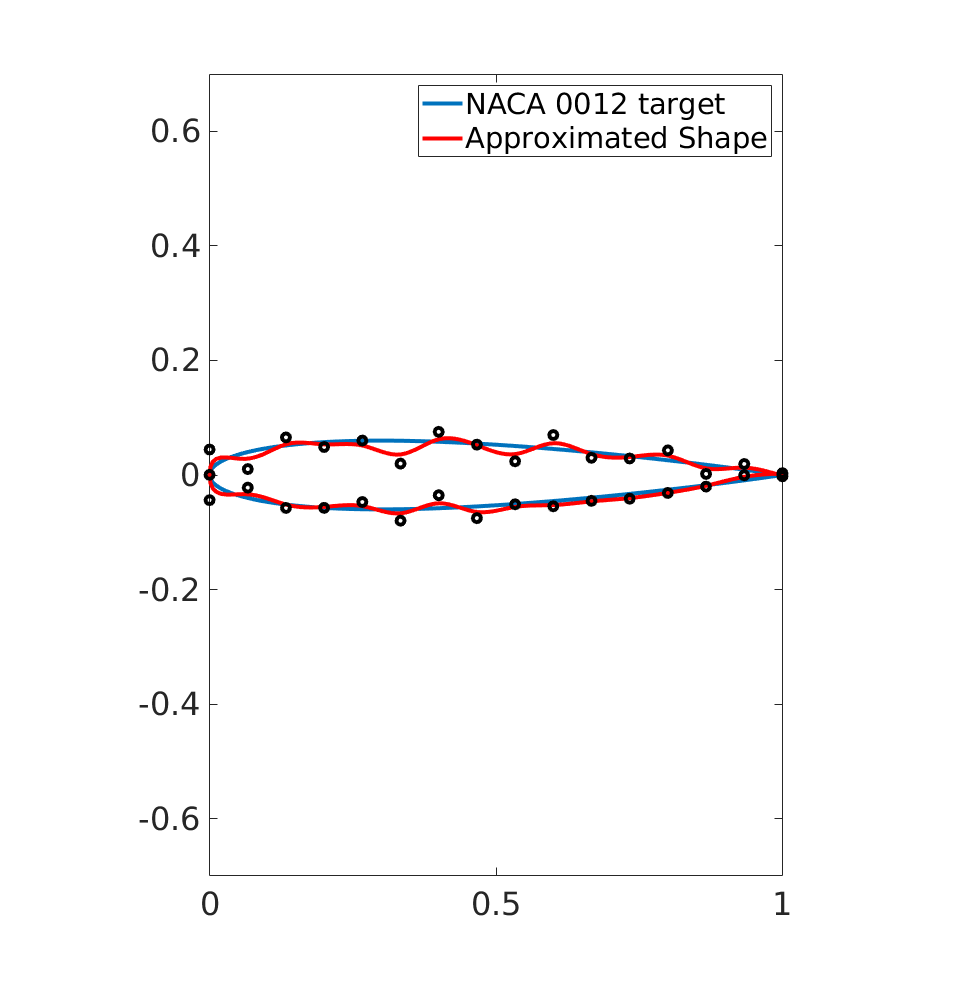
\includegraphics[width=0.45\textwidth]{img/Best_bit_GA_20_20000.png}
		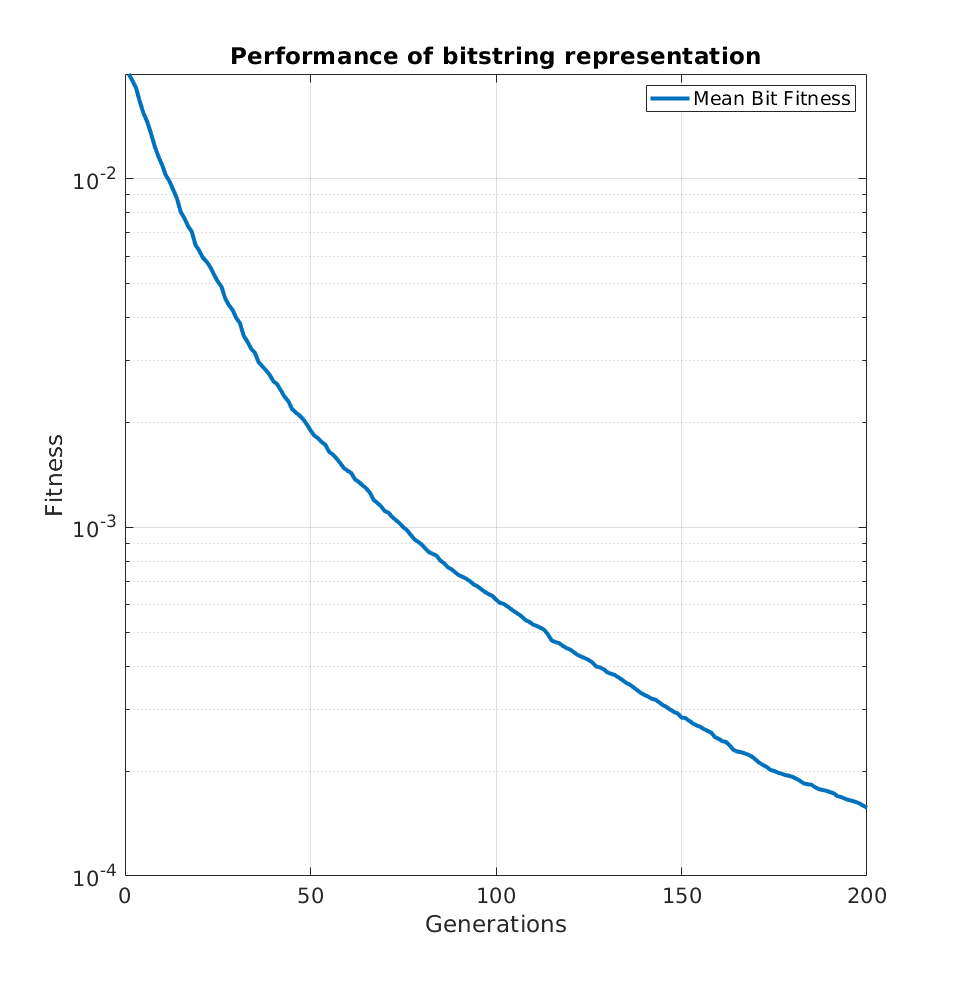
\includegraphics[width=0.45\textwidth]{img/GA_bit_fit.png}
		\caption{a) Performance of the GA having a bit string representation. b) Best individual over 20 runs. \label{fig:xxx1}}
	\end{figure}
	

	\item \textit{***Extra Credit***} Implement both encodings and compare them on matching task for \underline{one} of the shapes. Is one significantly better? Can you explain why?
	\\\color{blue}
	- Run-time:\\
	+ Real value representation: 330 seconds\\
	+ Bitstring representation: 335 seconds.\\
	Having a higher run-time for the bitstring was expected due to the many conversions that are required for the individuals in order to compute the crossover, mutation and fitness value calculation. \\
	
	As it can be appreciated from the resulting images, the bitstring representation obtained a much better result in comparison with the real-value representation. We looked for a concrete reason behind the better performance of the bitstring, but we only found that authors tend to refer to the bitstring as the optimal representation. But, we could not find an idea that could back up this claim. \\
	
	Perhaps, the way mutation occurs differently than the real value representation could be the key aspect of the better performance of the bitstring representation.
	 
	\color{black}
	
	\begin{figure}[http]
		\centering
		\begin{subfigure}[b]{.52\linewidth}
			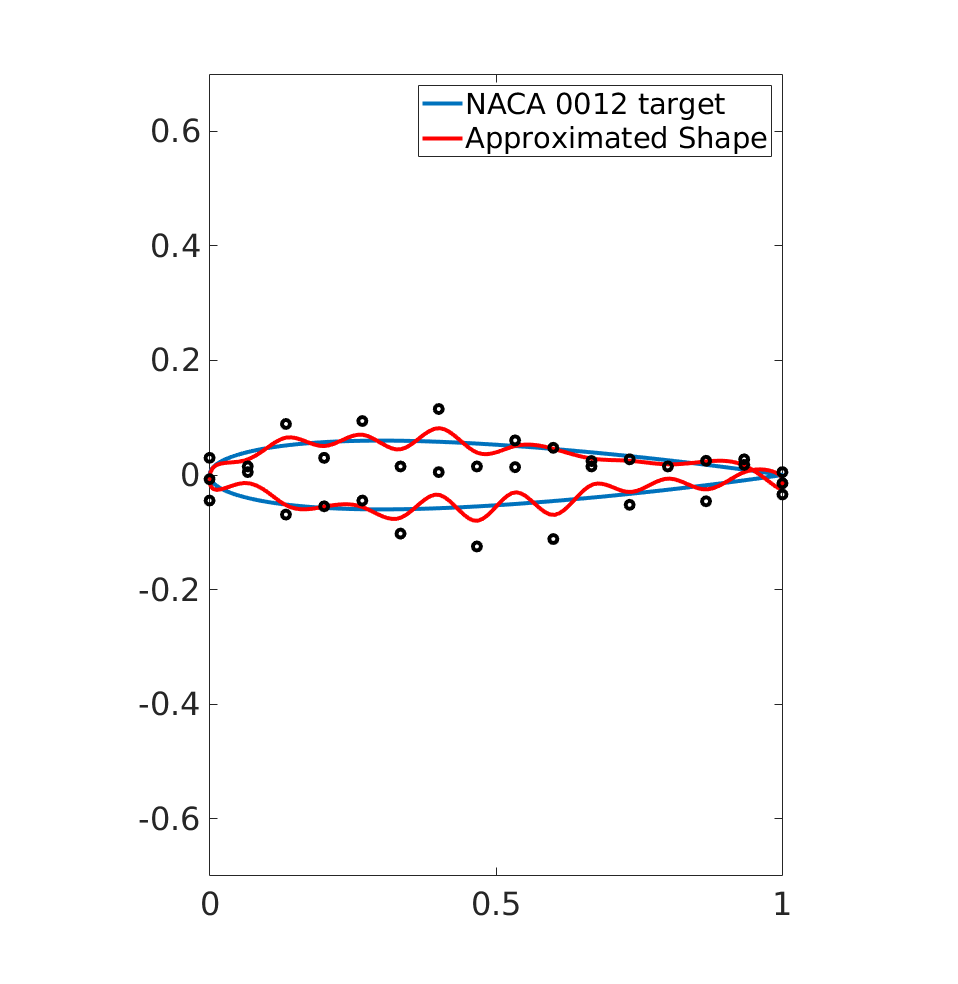
\includegraphics[scale = 0.3]{img/Best_real_GA_20_20000.png}
			\caption{Best individual for real value representation.}
			
		\end{subfigure}
		\hspace{1mm}
		\begin{subfigure}[b]{.45\linewidth}
			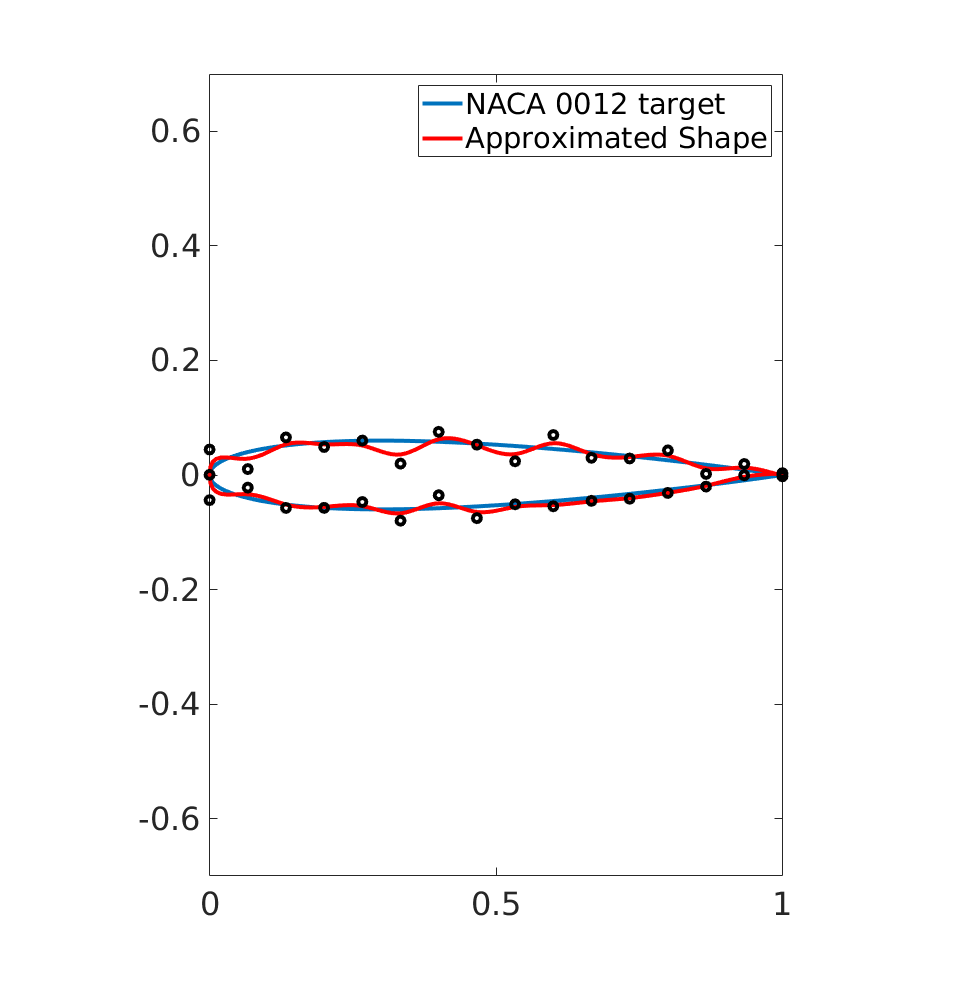
\includegraphics[scale=0.3]{img/Best_bit_GA_20_20000.png}
			\caption{Best individual for bitstring representation}\label{fig:tiger}
		\end{subfigure}
		
		\begin{subfigure}[b]{.45\linewidth}
			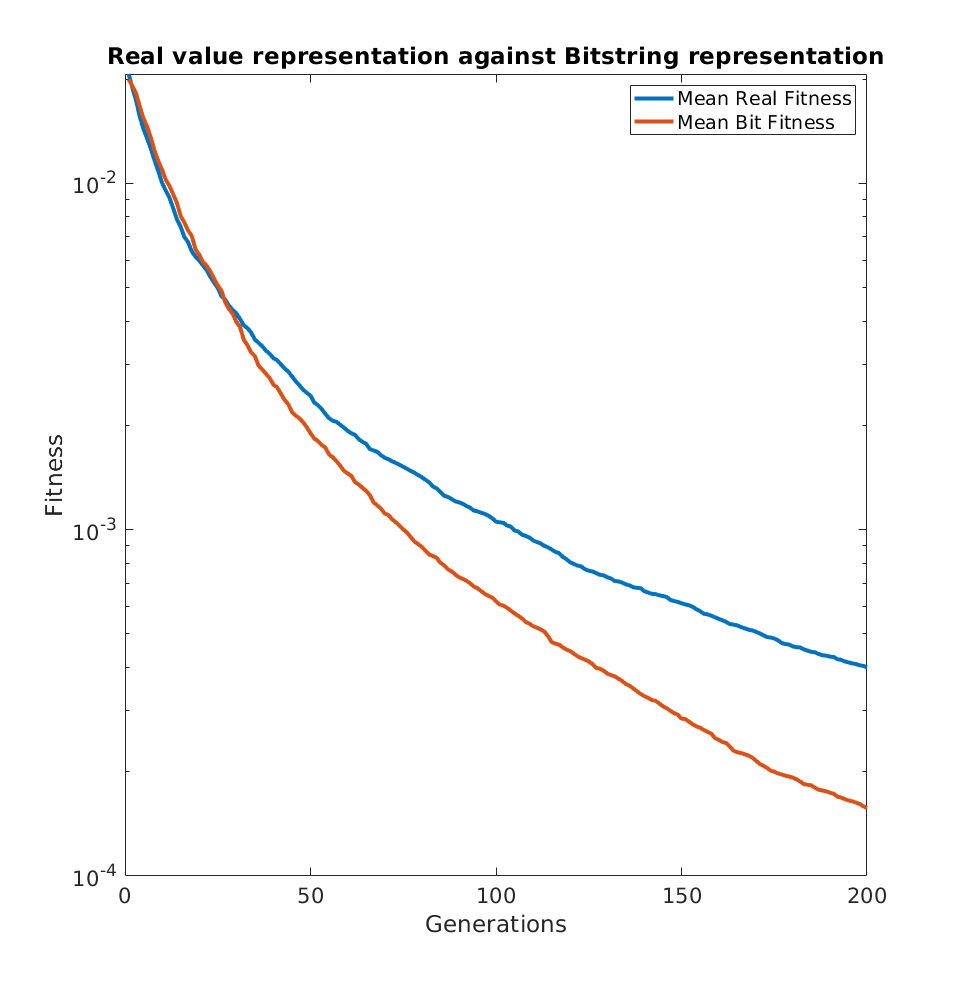
\includegraphics[scale = 0.3]{img/GA_real_vs_bit.png}
			\caption{Comparison of the mean fitness for real value representation and bitstring.. \label{fig:xxx1}}
			
		\end{subfigure}
		\caption{GA implementation over 20,000 evaluations}
	\end{figure}
	
\end{itemize}

\newpage
\subsection{Evolution Strategies}
\begin{itemize}
	\item CMA-ES is an advanced version of ES. As a first step implement a simple ES first. 
		\begin{itemize}
			\item In this ES mutation of all parameters should have equal strength which is adjusted by the 1/5th rule.\\(\textit{every N generations change mutation strength: if $>1/5$th of mutations resulted in an better fitness (i.e. a best solution) increase mutation strength, otherwise decrease mutation strength}). Test your implementation on \underline{one} of the shapes.
			\item Compare to your best GA. Is one significantly better than the other?
			\\\color{blue}\\
			\begin{figure}[http]
				
				\begin{subfigure}[b]{.50\linewidth}
					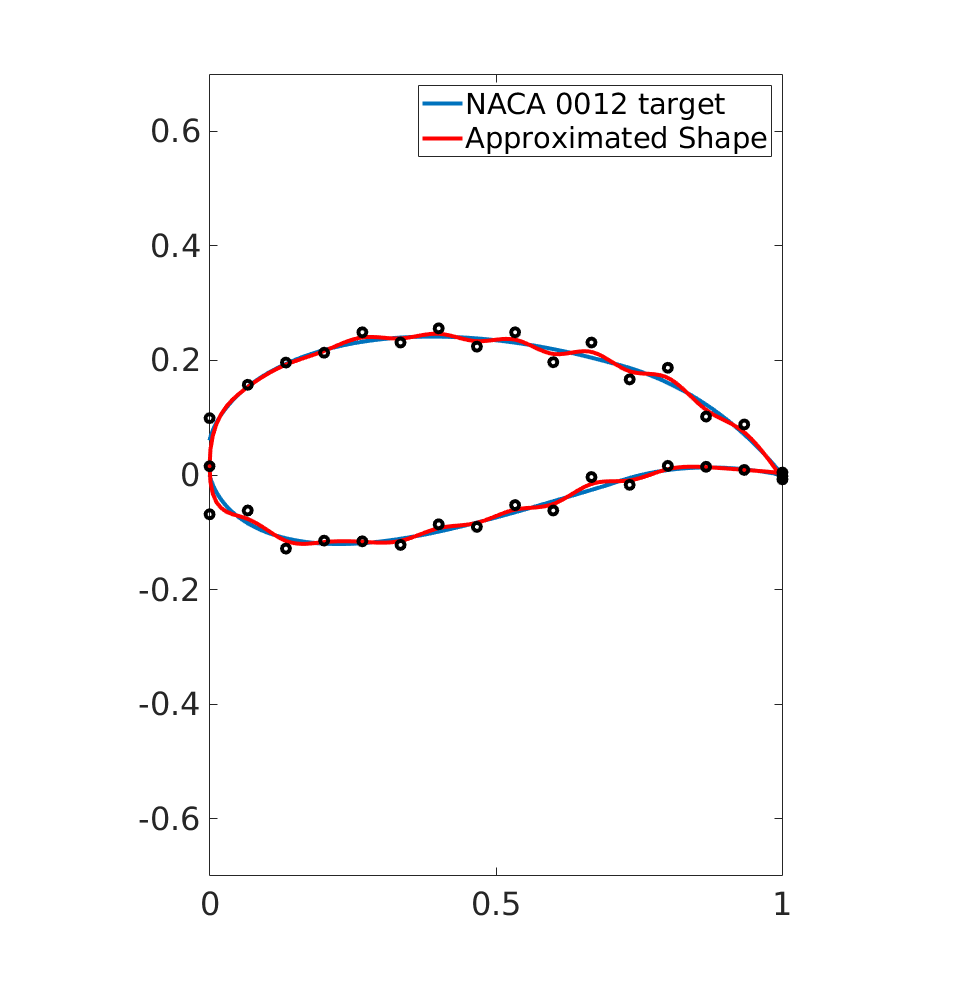
\includegraphics[scale=0.3]{img/GA_wing3_real.png}
					\caption{Best individual for GA real value representation}\label{fig:tiger}
				\end{subfigure}
				\hspace{2mm}
				\begin{subfigure}[b]{.45\linewidth}
					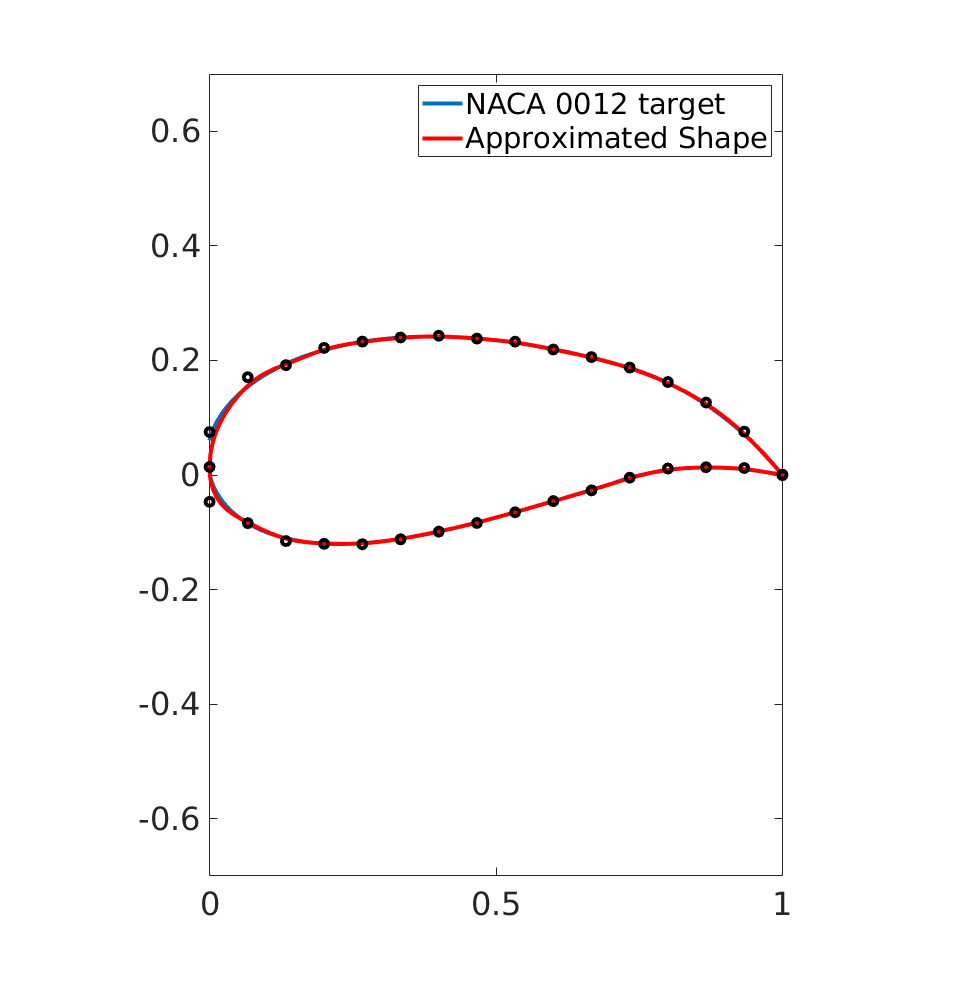
\includegraphics[scale = 0.3]{img/ES_wing3_mean.png}
					\caption{Mean individual for ES  \label{fig:xxx1}}
					
				\end{subfigure}
				\centering
				\begin{subfigure}[b]{.52\linewidth}
					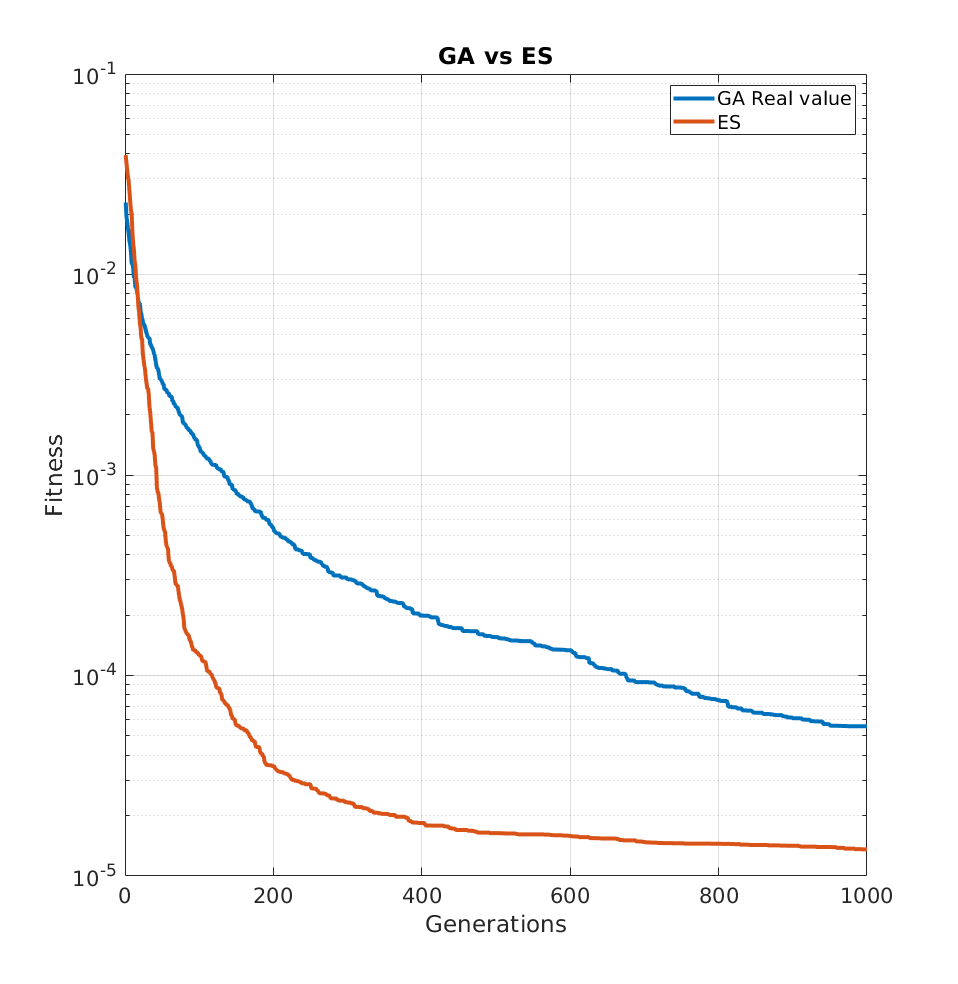
\includegraphics[scale = 0.3]{img/GA_vs_ES.png}
					\caption{Performance plot.}
					
				\end{subfigure}
				\caption{GA vs ES on wing 3 for 20 runs}
			\end{figure} 
			\color{black}
		\end{itemize}
	\item Now program CMA-ES \underline{without evolution paths}.
	\begin{itemize}
		\item Compare to your ES results. Is a there a significant improvement?
		\\\color{blue}\\
		\begin{figure}[http]
			
			\begin{subfigure}[b]{.50\linewidth}
				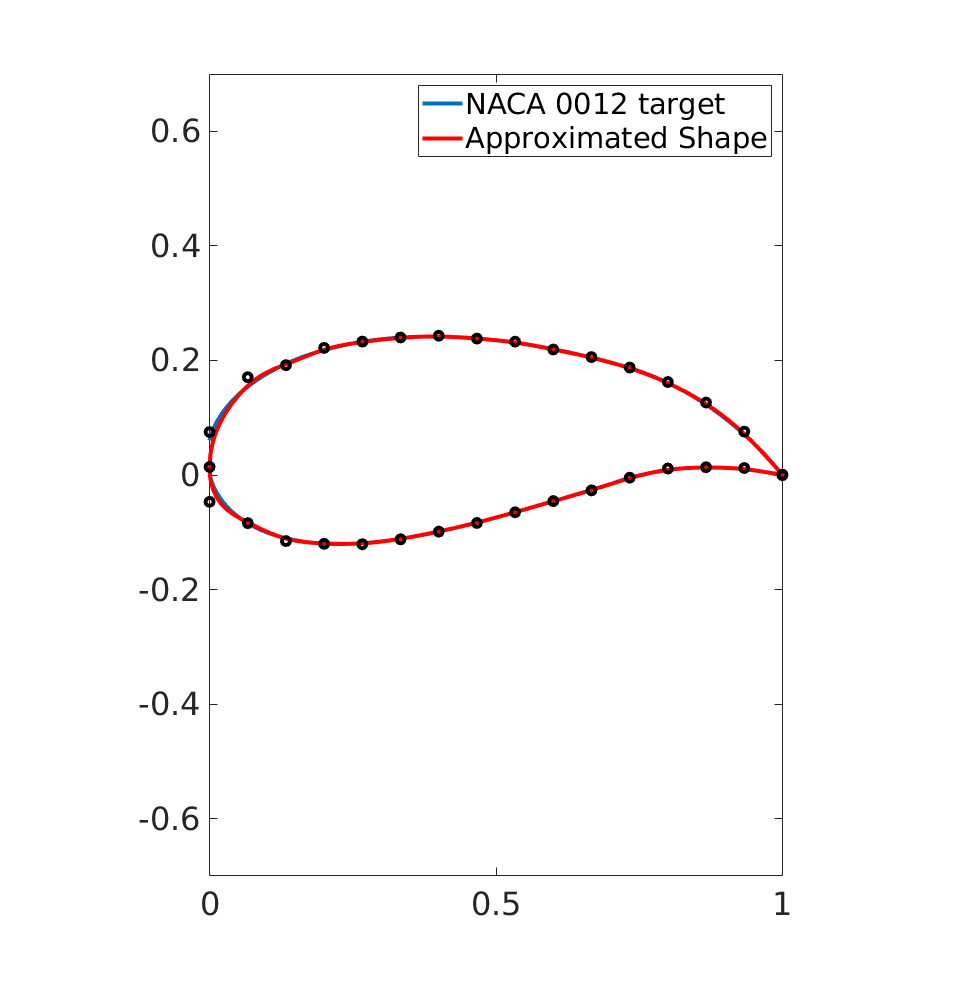
\includegraphics[scale=0.3]{img/ES_wing3_mean.png}
				\caption{Mean individual for ES}\label{fig:tiger}
			\end{subfigure}
			\hspace{2mm}
			\begin{subfigure}[b]{.45\linewidth}
				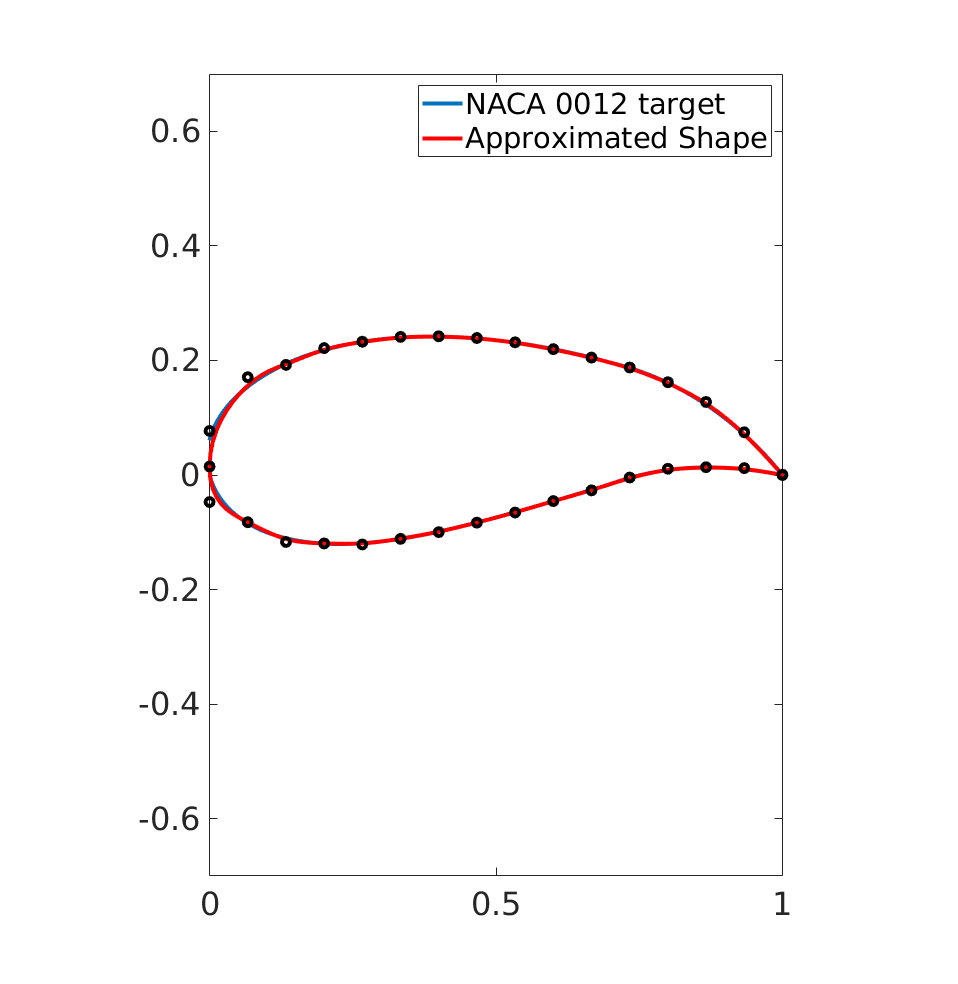
\includegraphics[scale = 0.3]{img/CMA_ES_N_wing3_mean.png}
				\caption{Mean individual for CMA-ES without evolutionary paths  \label{fig:xxx1}}
				
			\end{subfigure}
			\centering
			\begin{subfigure}[b]{.52\linewidth}
				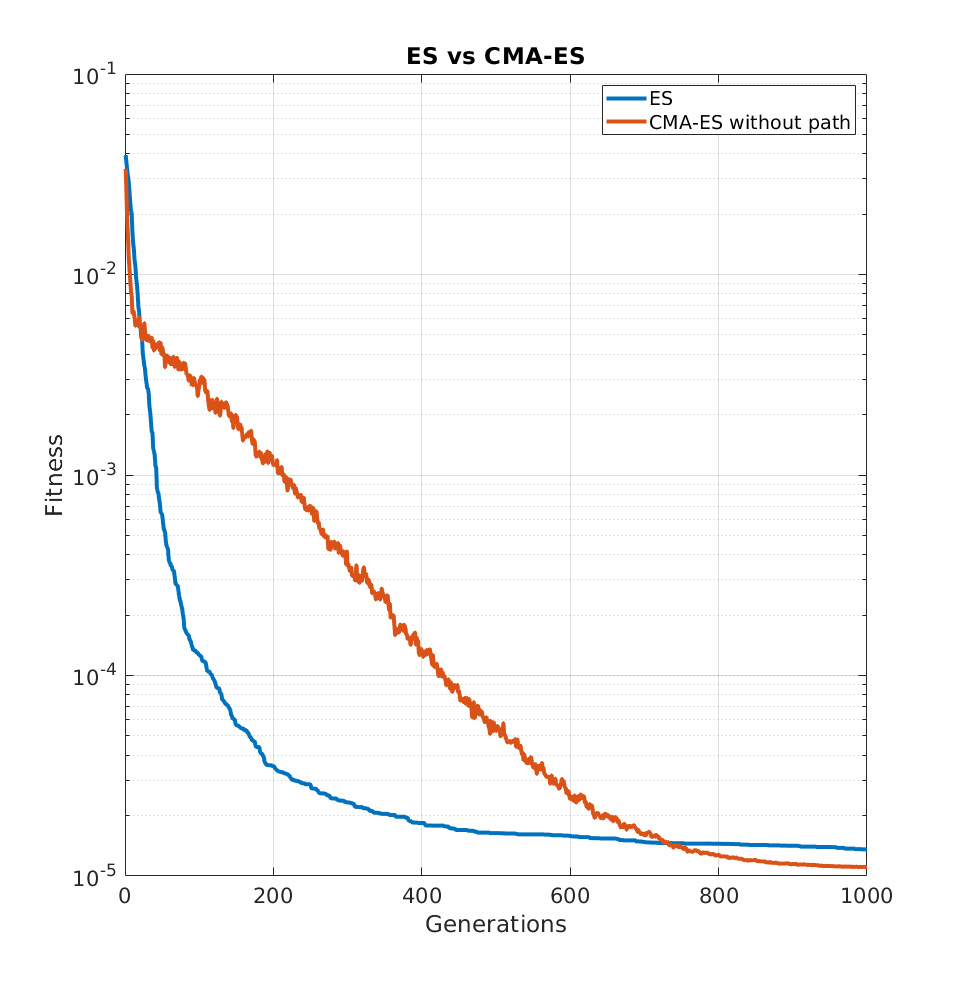
\includegraphics[scale = 0.3]{img/CMA_ES_vs_ES.png}
				\caption{Performance plot.}
				
			\end{subfigure}
			\caption{ES vs CMA-ES without evolutionary paths on wing 3 for 20 runs}
		\end{figure} 
		\color{black}	
	\end{itemize}

	\item \textit{***Extra Credit***} Now program CMA-ES \underline{with evolution paths}.
		\begin{itemize}
		\item Compare to your previous CMA-ES results. Is a there a significant improvement?
		\\\color{blue}\\
		\begin{figure}[http]
			
			\begin{subfigure}[b]{.50\linewidth}
				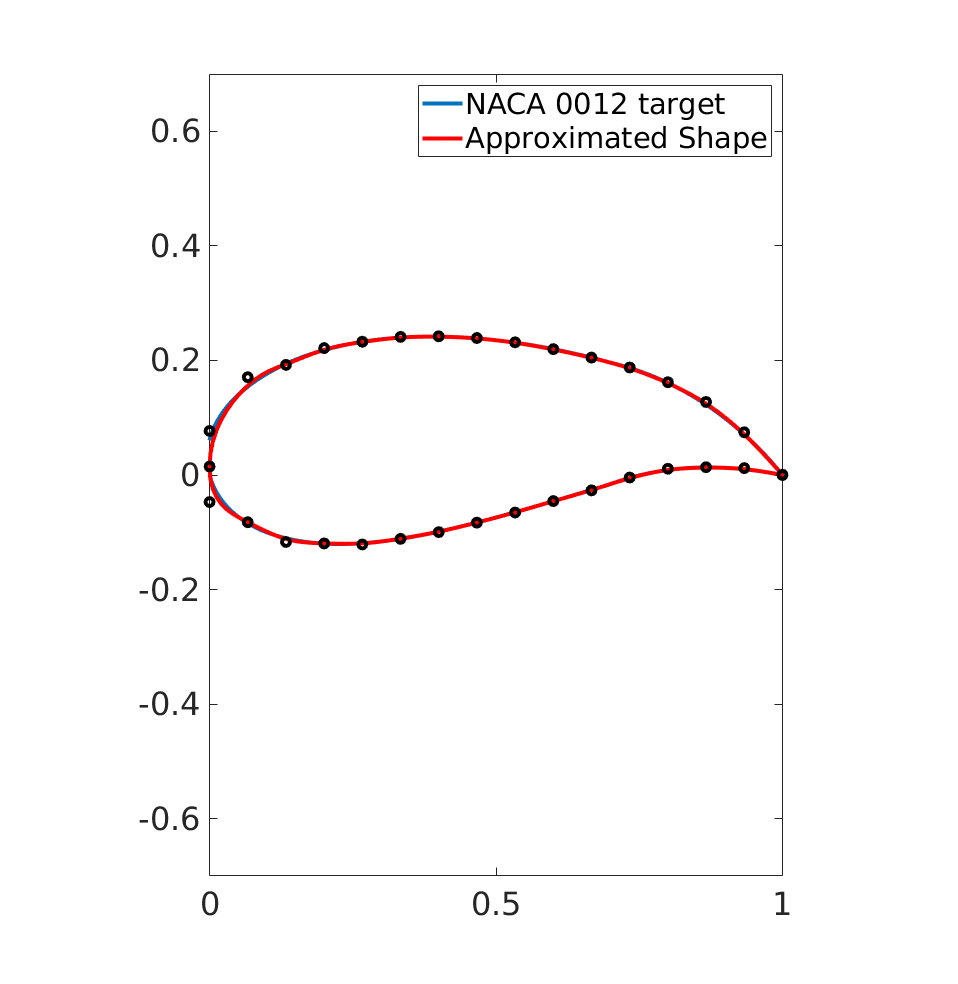
\includegraphics[scale=0.3]{img/CMA_ES_N_wing3_mean.png}
				\caption{Mean individual for CMA-ES without evolutionary paths}\label{fig:tiger}
			\end{subfigure}
			\hspace{2mm}
			\begin{subfigure}[b]{.45\linewidth}
				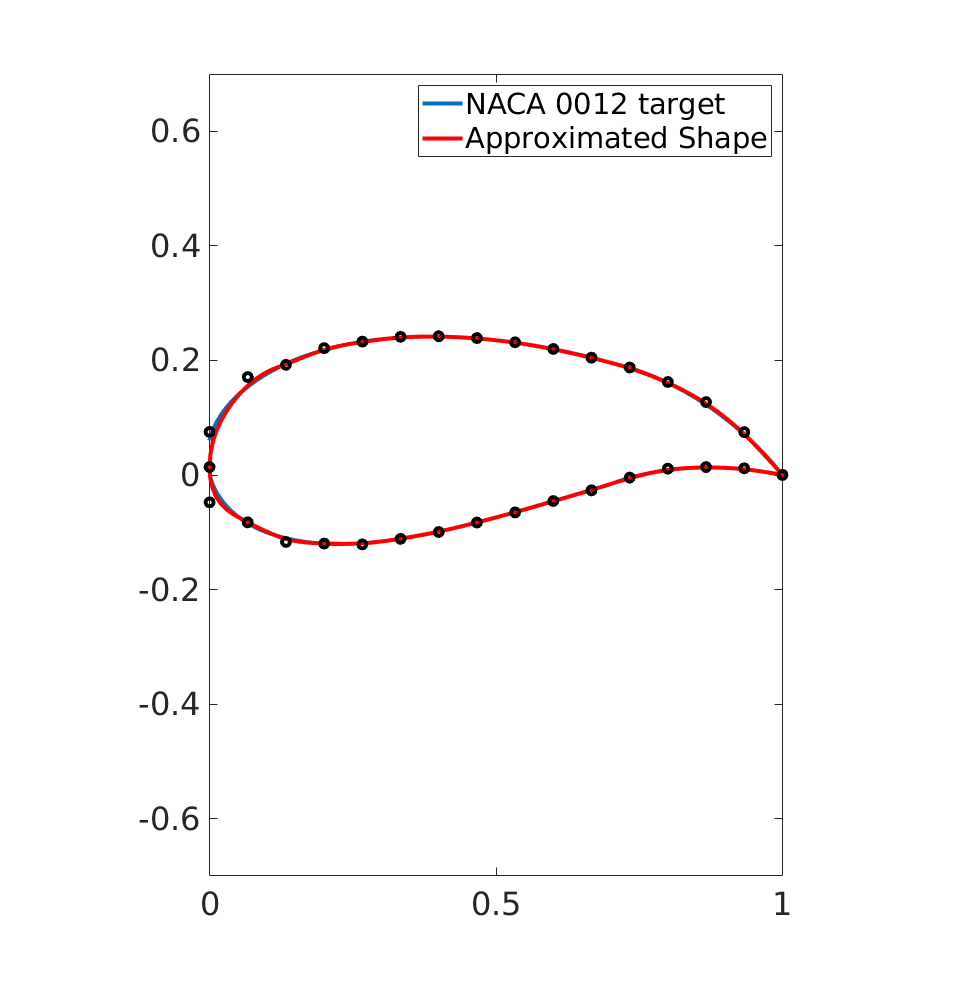
\includegraphics[scale = 0.3]{img/CMA_ES_wing3_mean.png}
				\caption{Mean individual for CMA-ES with evolutionary paths  \label{fig:xxx1}}
				
			\end{subfigure}
			\centering
			\begin{subfigure}[b]{.52\linewidth}
				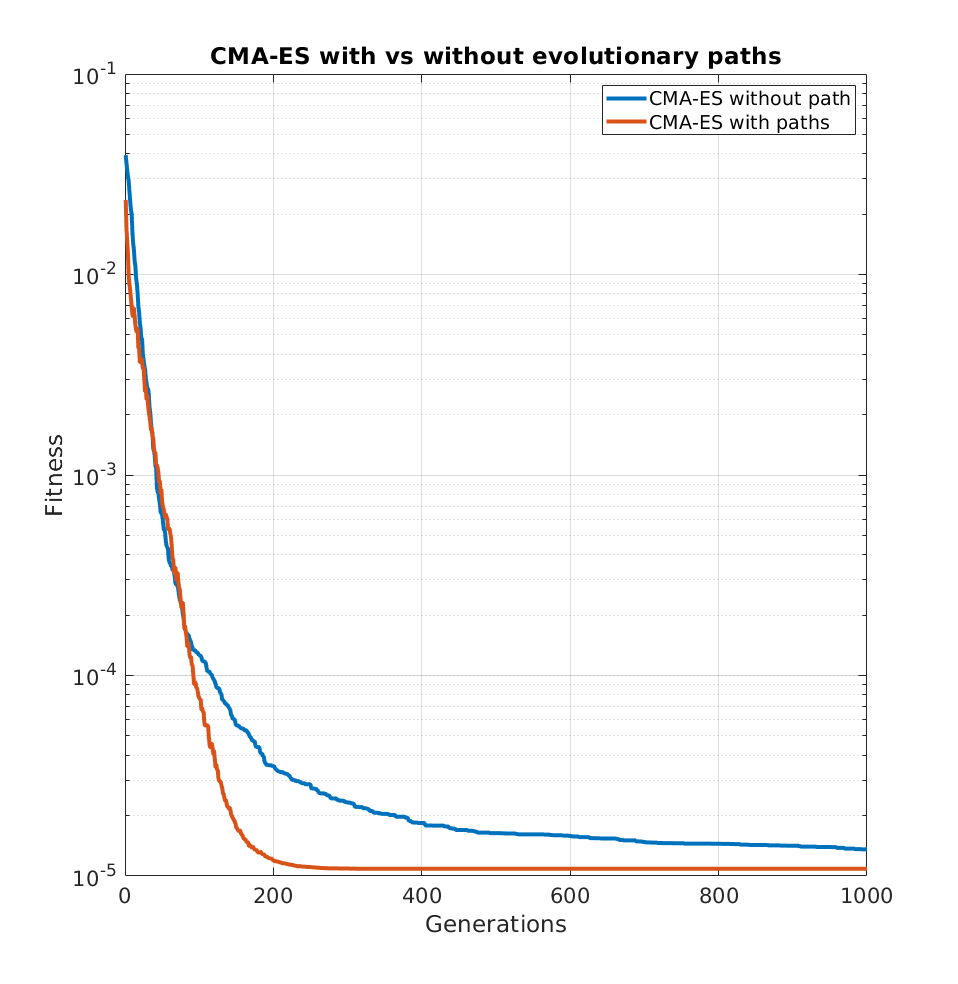
\includegraphics[scale = 0.3]{img/CMAES_vs_CMAES.png}
				\caption{Performance plot.}
				
			\end{subfigure}
			\caption{CMA-ES with vs without evolutionary paths on wing 3 for 20 runs}
		\end{figure} 
		\color{black}
		\end{itemize}
\end{itemize}

\newpage
\subsection{Comparisons}
Produce one plot which shows the performance of each algorithm. Run each algorthm 20 times on each shape (NACA airfoil shapes: 0012, 5522, 9735), with a budget of 20,000 function evaluations. For each run record the best ever found individual at each evaluation. For each algorithm plot the median fitness of this best ever individual. This may take some time, write a script to run and collect this data. The following should be on this plot (leaving out any algorithms you chose not to implement):
\begin{enumerate}
	\item Real-Valued GA
	\item ES
	\item CMA-ES (without evolution paths)
	\item CMA-ES (with evolution paths)
\end{enumerate}	
	\begin{figure}[h!]
		\centering
		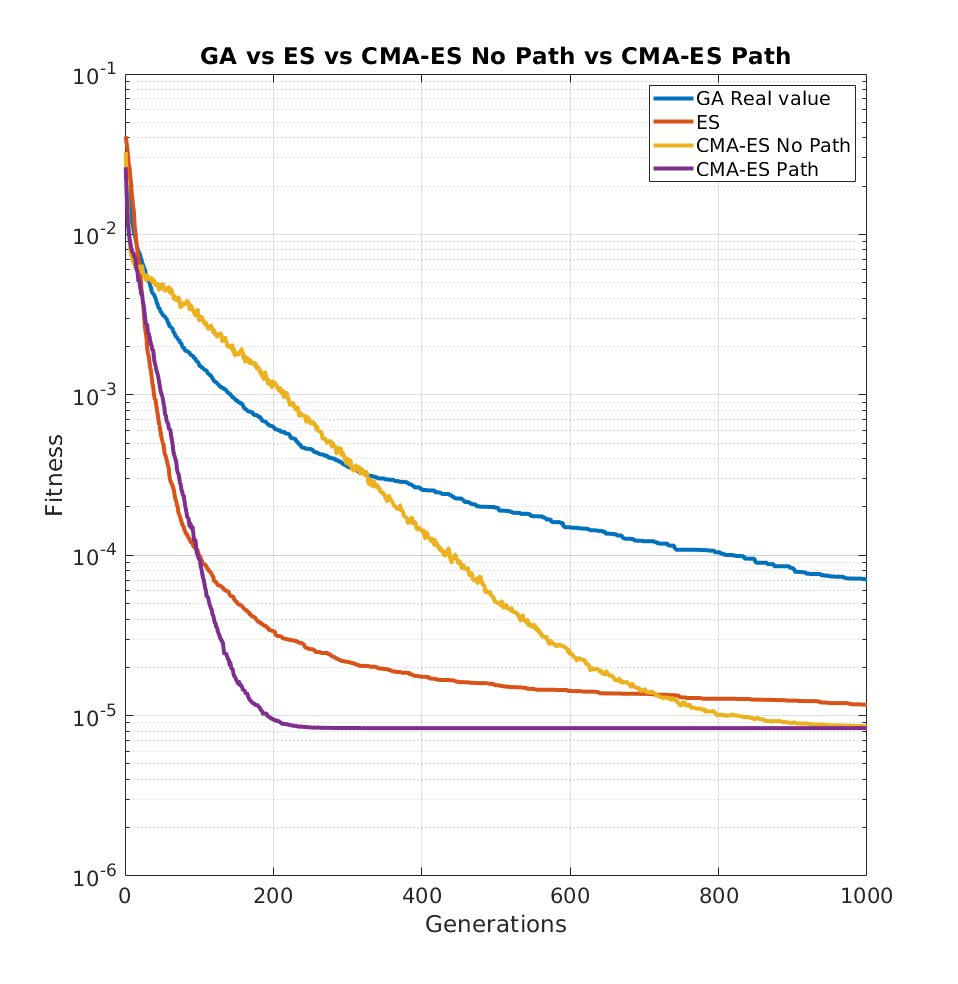
\includegraphics[scale=0.5]{img/all_for_one.png}
		\caption{Performance comparison between:\\
			a) GA with real value representation\\
			b) ES with 1/5 rule\\
			c) CMA-ES without evolution paths\\
			d) CMA-ES with evolution paths.\label{fig:xxx1}}
	\end{figure}







\end{document}










